\section{Расчет биологической защиты} %TODO: убрать для репорта
\subsection{Постановка задачи}
Необходимо рассчитать дозу облучения при стационарном режиме работы ЯЭУ ВВЭР-1000 за биологической защитой

\subsection{Построение расчетной модели биологической защиты}
Для формирования расчетной модели рассмотрим разомкнутую компоновку элементов и помещений ЯЭУ с РУ ВВЭР-1000. Такая компоновка предполагает разделения реакторного и машинного залов в разные здания, что позволяет локализовать возможную аварию и обеспечить большую безопасность.

\begin{figure}[H]
	\begin{center}
		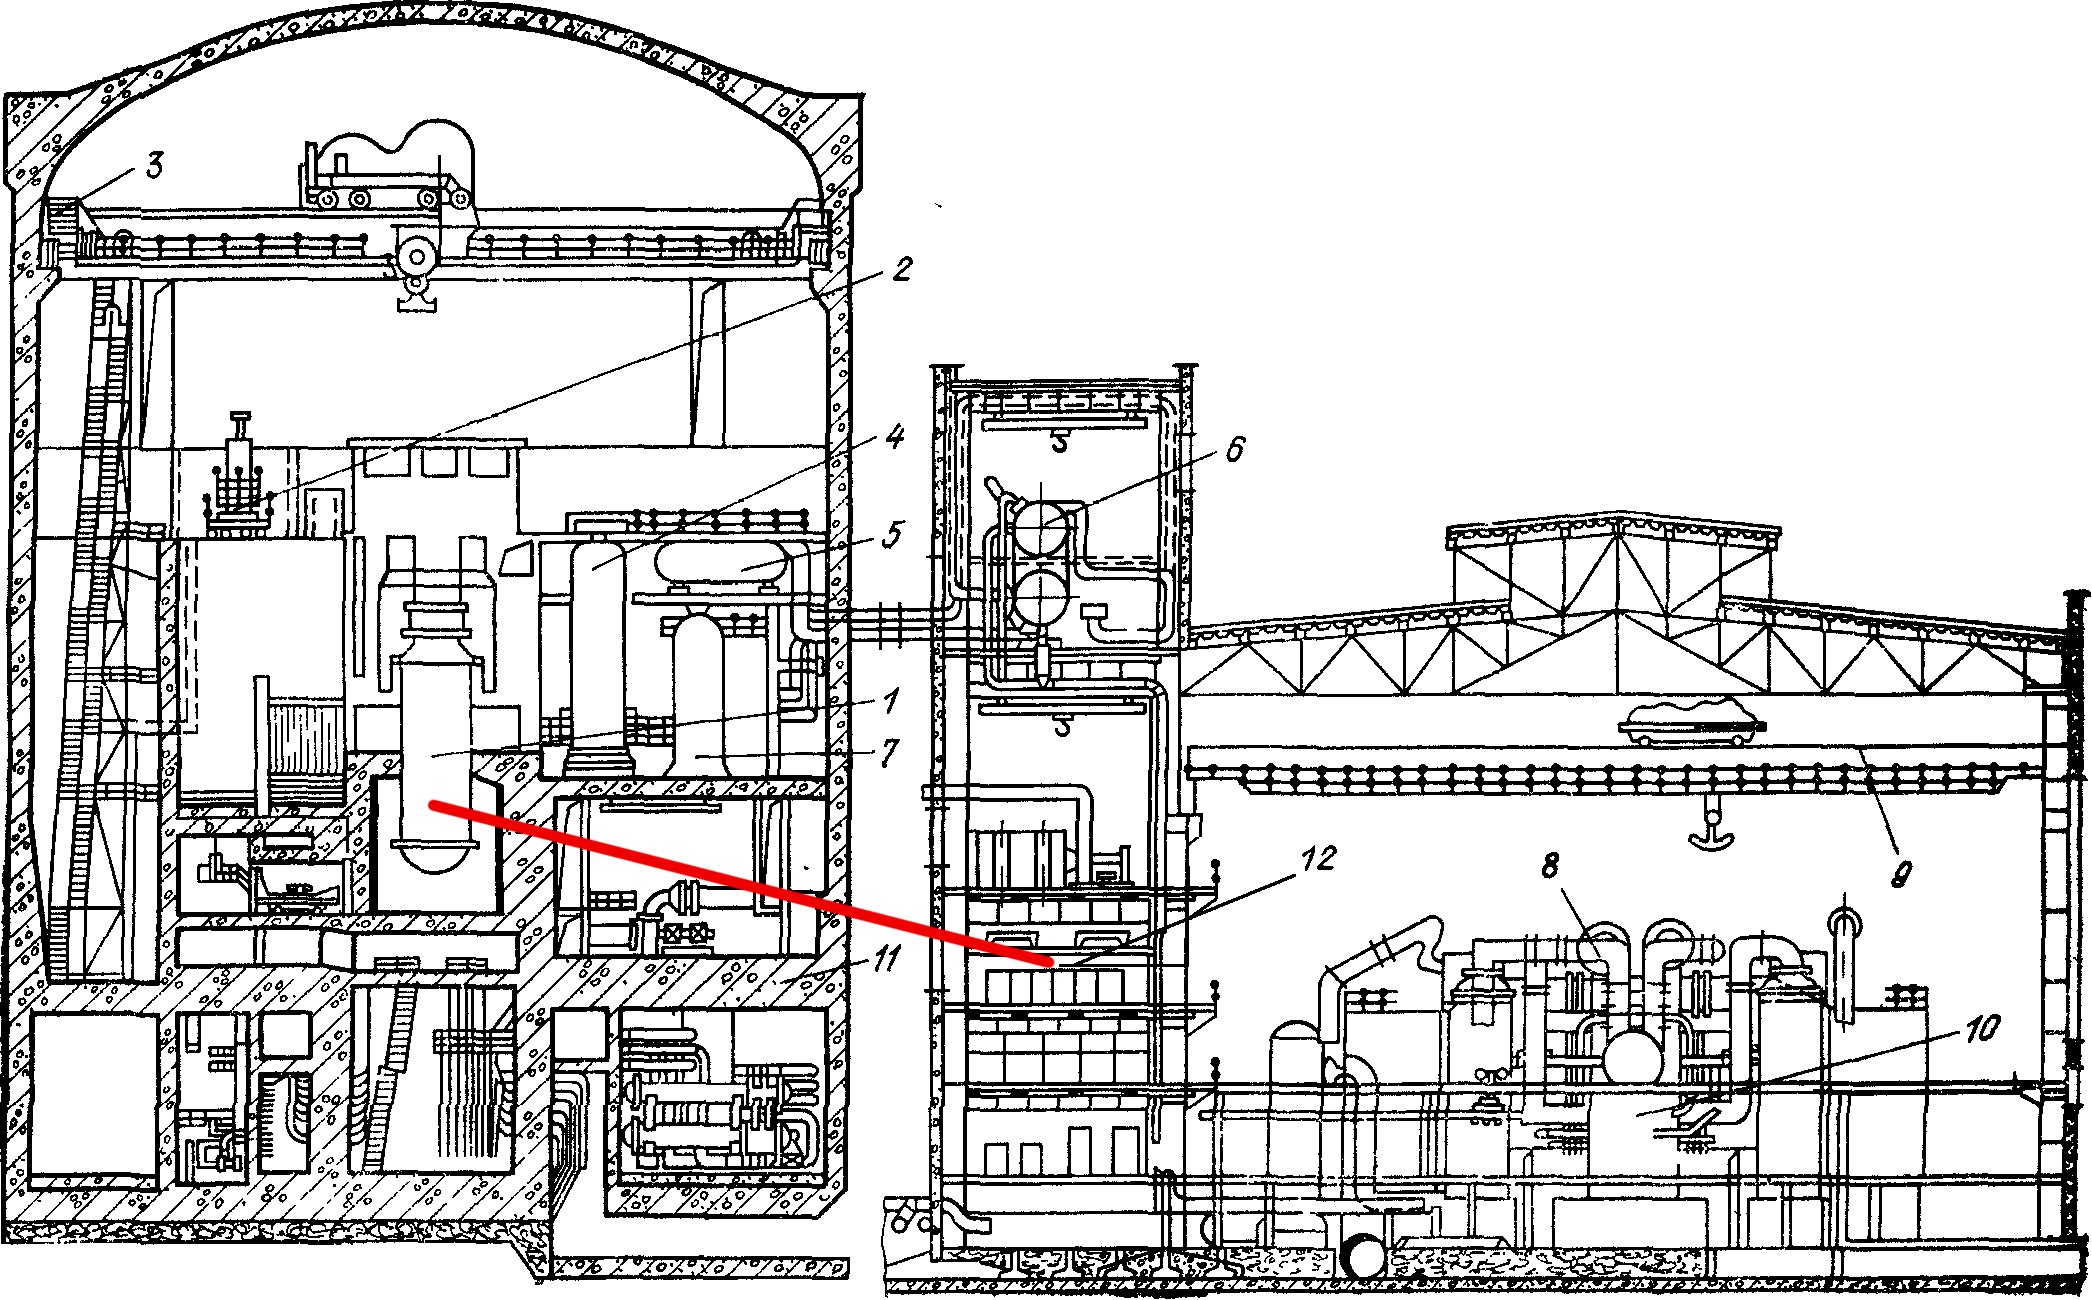
\includegraphics{razrez_bio.png}
		\caption{
			Общая компоновка энергоблока с РУ ВВЭР-1000 разомкнутой компоновки (Южно-Украинская АЭС) \cite{МонаховА.С1986Аэси}: \\
			1 — реактор; 2 — машина для перегрузки топлива; 3 — подъемный кран реакторного отделения; 4 — компенсатор давления, 5 — барботер; 6 — деаэратор; 7 — гидроемкость, 8 — турбогенератор; 9 — подъемный кран машинного зала; 10 — регенеративные подогреватели, 11 —  защитная оболочка
		}
		\label{pic:razrez_bio} % название для ссылок внутри кода
	\end{center}
\end{figure}
% Монахов Атомные электрические станции и их технологическое оборудование

\paragraph{Элементы компоновки вокруг реактора}

Рассмотрим основные элементы защиты, внешние по отношению к ВВЭР-1000 в сборе. Корпус реактора установливается в \textit{бетонную шахту} (рис \ref{pic:beton_shakhta}), которая играет роль основной опоры и крепления реактора с учетом сейсмических нагрузкок, а также биологической защиты от излучения со стороны АЗ. Между корпусом реактора и шахтой имеется кольцевой зазор, предназначенный для периодического контроля металла корпуса в связи с требованиями правил. Шахта резделена по высоте на два объема разделительным сильфоном: 
\begin{itemize}
	\item Верхний, снабжен гидрозатвором и соединяется с бассейном выдержки. При перегрузке верхний объем шахты вместе с бассейном заливается водой.
	\item Нижний, условно разделяемый фермой опорной на шахту зоны патрубков и шахту цилиндрической части корпуса. Соединяется проемом, снабженным герметичной дверью, с помещением для машины осмотра корпуса.
\end{itemize}
В помещении зоны патрубков
биологическая защита выполнена из металлических коробов, заполненных специальным составом, в который входят серпентинитовая галя, кристаллический карбид бора, дробь чугунная литая. В районе активной зоны применяется «сухая» защита, которая представляет из себя слой серпентинитового бетона толщиной
720 мм и высотой 4,7 м, облицованного металлической оболочкой. Такой бетон обладает высокой радиационной стойкостью, что позволяет удовлетворить требования по нейтронной защите. \cite{лескин2011физические}

\begin{figure}[H]
	\begin{center}
		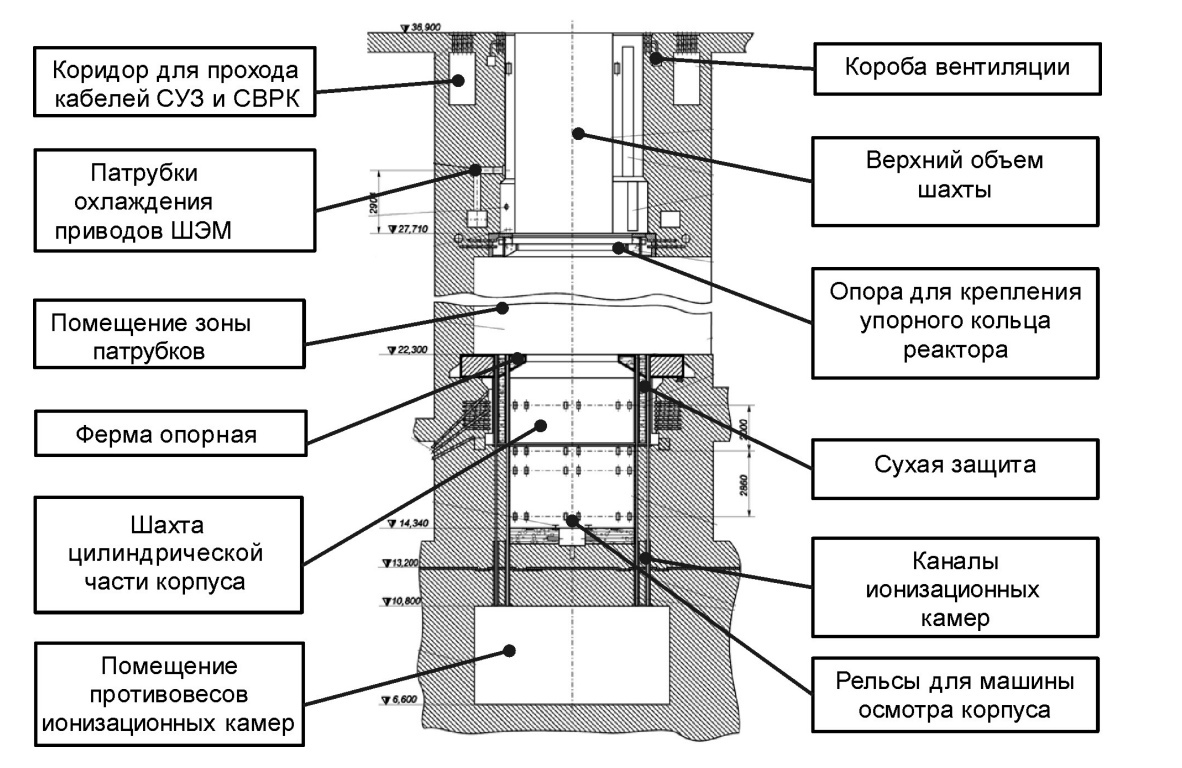
\includegraphics[scale=0.4]{beton.jpg}
		\caption{
			Бетонная шахта реактора 
		}
		\label{pic:beton_shakhta} % название для ссылок внутри кода
	\end{center}
\end{figure}

Все оборудование первого контура заключено в цилиндрическую оболочку, в верхней части которой расположен грузоподъемный поворотный кран. Между реакторным и машинным залами располагается этажерка электротехнических устройств, где размещены также деаэраторы и различные лаборатории.

\paragraph{Корпус и внутрикорпусные элементы компоновки} Корпус представляет собой вертикальный герметичный сосуд
цилиндрической формы с эллиптическими днищем и крышкой  с наружним диаметром 4535 мм, высотой 10.897 м и толщиной 192 мм в цилиндрической части и 210 мм в районе патрубков \cite{лескин2011физические}. В качестве основного материала используется сталь сталь 15Х2НМФА. е. Вся внутренняя поверхность корпуса покрыта
антикоррозионной наплавкой из нержавеющей стали толщиной не
менее 8 мм. В местах соприкосновения корпуса с крышкой, шахтой, уплотнительными прокладками, в местах приварки
кронштейнов, деталей крепления трубок КИП, на поверхности разделительного кольца выполнена наплавка толщиной не менее
15 мм. Внутрь реактора также устанавливается шахта, которая  представляет собой цилиндрическую обечайку с фланцем и эллиптическим днищем, в котором закреплены 163 опорные
трубы (стаканы) с шагом 236 мм, верхние части которых образуют
опорную плиту для установки и дистанционирования кассет активной зоны. Материал шахты – сталь 08Х18Н10Т толщиной 55 мм.

\paragraph{Устройство твэла} Твэл ядерного реактора ВВЭР-1000 представляет собой трубку, заполненную таблетками из двуокиси урана UO2 и герметично уплотненную концевыми деталями на сварке. Трубка твэла изготовлена из циркония, легированного 1 \% ниобия. Наружный диаметр трубки твэла 9.1±0.05 мм, ее толщина 0.65±0.03 мм, а внутренний диаметр 7.72+0.08 мм.
В эту трубку с зазором 0.19–0.32 мм на диаметр помещены таблетки двуокиси урана высотой (длиной) 20 мм и диаметром 7.57±0.04 мм. В середине этих таблеток имеются отверстия диаметром 1.5 мм, а края таблеток скруглены фасками. Общая длина столба этих таблеток в твэле составляет 3530 мм. Все размеры указаны для холодного состояния. Длина трубки твэла составляет 3800 мм, поэтому положение столба топливных таблеток в твэле зафиксировано разрезными втулками из нержавеющей стали и пружиной, не препятствующими тепловым перемещениям. Вид твэла приведён на рис. \ref{pic:tvel} \cite{ТвэлТерновых}

\begin{figure}[H]
    \begin{center}
        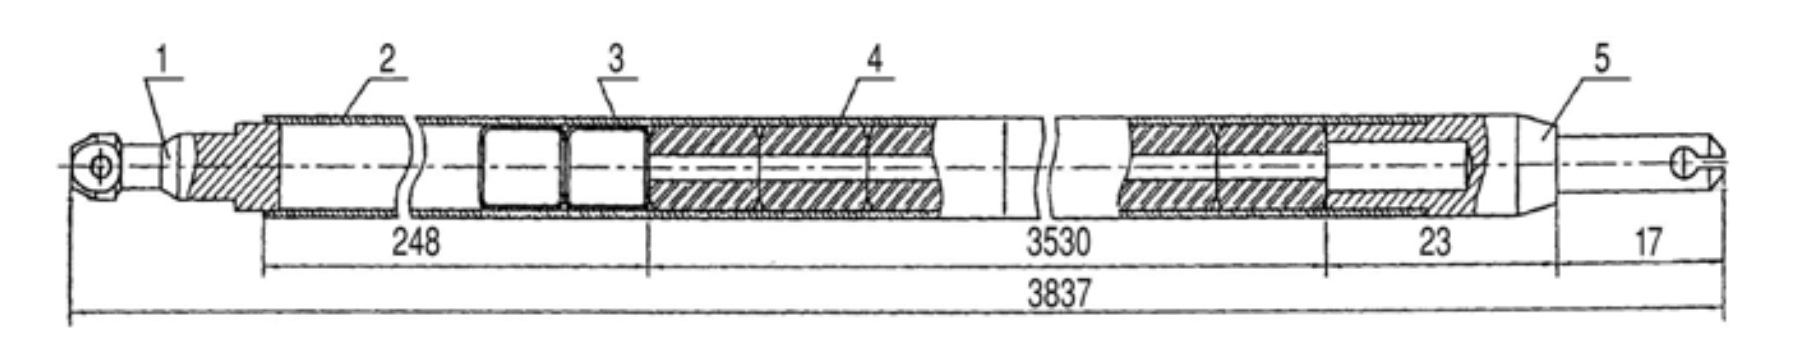
\includegraphics[scale=0.3]{tvel.jpg}
        \caption{
                Тепловыделяющий элемент: 1 – заглушка верхняя; 2 – оболочка; 3 – фиксатор; 4 – таблетка; 5 – заглушка нижняя
        }
        \label{pic:tvel}
    \end{center}
\end{figure}

Преимущество циркония заключается в удачном сочетании ядерных и физических характеристик с механическими и коррозионными свойствами. Цирконий коррозионно стоек в большинстве сред, применяемых в качестве теплоносителей ядерных реакторов, и достаточно технологичен.

Естественная радиоактивность одной свежей ТВС составляет $1.8 \cdot 10^{10}$ Бк., гамма- излучение на поверхности около 0.2 бэр/ч.


\paragraph{Построение одномерной модели} В качестве помещения постоянного пребывания персонала рассматривается блочный щит управления, расположенный в этажерке электроустройств (цифра 12 на рис. \ref{pic:obsh}). Также в этажерке электроустройств размещаются распределительные устройства сетей электропитания двигателей электростанции, аккумуляторные батареи, трансформаторы и т. д.
Для построения расчетной модели был определен ряд значимых элементов конструкции реакторной установки с точки зрения нейтронной защиты. От активной зоны рассматриваемое помещение отделено внутрикорпусными элементами, такими как оболочка твэла, внутрикорпусная шахта; корпусом, бетонной внешней шахтой, внешней бетонной оболочкой реактора и бетонной стеной машинного зала. Суммарный слой бетона складывается из 3 м основания гермооболочки, 0.72 м сухой защиты шахты, 1.5 м шахты и 0.5 м стены машинного зала перед этажеркой.
Основная доля нейтронного излучения в реакторе приходится на нейтроны теплового спектра. Для таких энергий хрошими поглотителями являются кадмий, графит, бетон. 
Присутствующее гамма-излучение для своего эффективного поглощения требует свинец и подобные высокоплотные материалы. Таким образом были выбран слои биологической защиты, представленные в таблице \ref{tabular:bio-sec-layers}:

\begin{table}[H]
	\caption{Слои биологической защиты}
	\begin{center}
        \begin{tabular}{|l|c|c|c|}
        \toprule
         Название & Материал & Размер & Плотность, $\text{г}/\text{см}^3$ \\ 
         \midrule
         \hline
         Оболочка ТВЭЛ & Zr1Nb & 0.65 мм & 6.55\\ 
         \hline
         Внутрикорпусная шахта & сталь 08Х18Н10Т & 55 мм & 7.9 \\ 
         \hline
         Корпус & сталь 15Х2НМФА & 192.5 мм & 7.8 \\ 
         \hline
         Бетонная шахта + гермооболочка + стена & бетон & 5720 мм & 2.35 \\ 
         %\hline
         %Герметичная оболочка & бетон &  & 2.5 \\ 
         \bottomrule
		\end{tabular}
		\label{tabular:bio-sec-layers}
	\end{center}
\end{table}

\subsection{Расчет дозы нейтронов из активной зоны реактора}

\begin{table}[H]
	\caption{Основные нейтронно-физические параметры}
	\begin{center}
        \begin{tabular}{|l|c|}
        \toprule
         Параметр & Значение \\ 
         \midrule
         \hline
         Тепловая мощность реактора, МВт & $2.904 \cdot 10^3$ \\ 
         \hline
         Средняя энергия, выделяющаяся в одной реакции деления, МэВ &  \\ 
         \hline
         Среднее число нейтронов деления на середину кампани & \\
         \hline
         Коэффициент размножения &  \\ 
         \hline
         Доля нейтронов спектра деления в спектре утечки &  \\ 
         \hline
         Среднее число гамма-квантов деления на середину кампании &  \\ 
         \bottomrule
		\end{tabular}
		\label{tabular:turbine}
	\end{center}
\end{table}